
\section{Results - Simulated Data}
\label{mmf-sec:simulated data}
\todo[inline]{probably make results its own section and then split into simulated and real world}
Just like in \autoref{ch:variantcalling}, the novelty of the approach leads to the issue of no gold standard dataset, with which to evaluate the performance of a new method. While there are low coverage WGS datasets of cancer patients, none of them have validated signatures associated with them. So again simulated data is the optimal starting point to allow both optimisation of parameters as well as granular detection of artefacts which can originate from any step starting from sequencing over mapping to the signature deconvolution. 

\subsection{Sequencing errors - there is always a cleaner data}
\label{mmf-sec:cleanSim}
To judge the ability of our approach to filter out sequencing errors, we first simulated ``clean`` sequencing reads with neither germline or somatic variants with the ART simulation suite \cite{Huang2011}. As current estimates of Illumina sequencing is in the range of 1 in 666 to 1 in 1149 \cite{Stoler2021} which is significantly higher than even the highest tumour mutational burdens of  cancers (melanoma: 1 in 5k; tobacco smoking lung cancer: 1 in 100k) it is very important to be able to eliminate as much of the  background noise of sequencing errors as possible.

\begin{figure}[!ht]
\centering
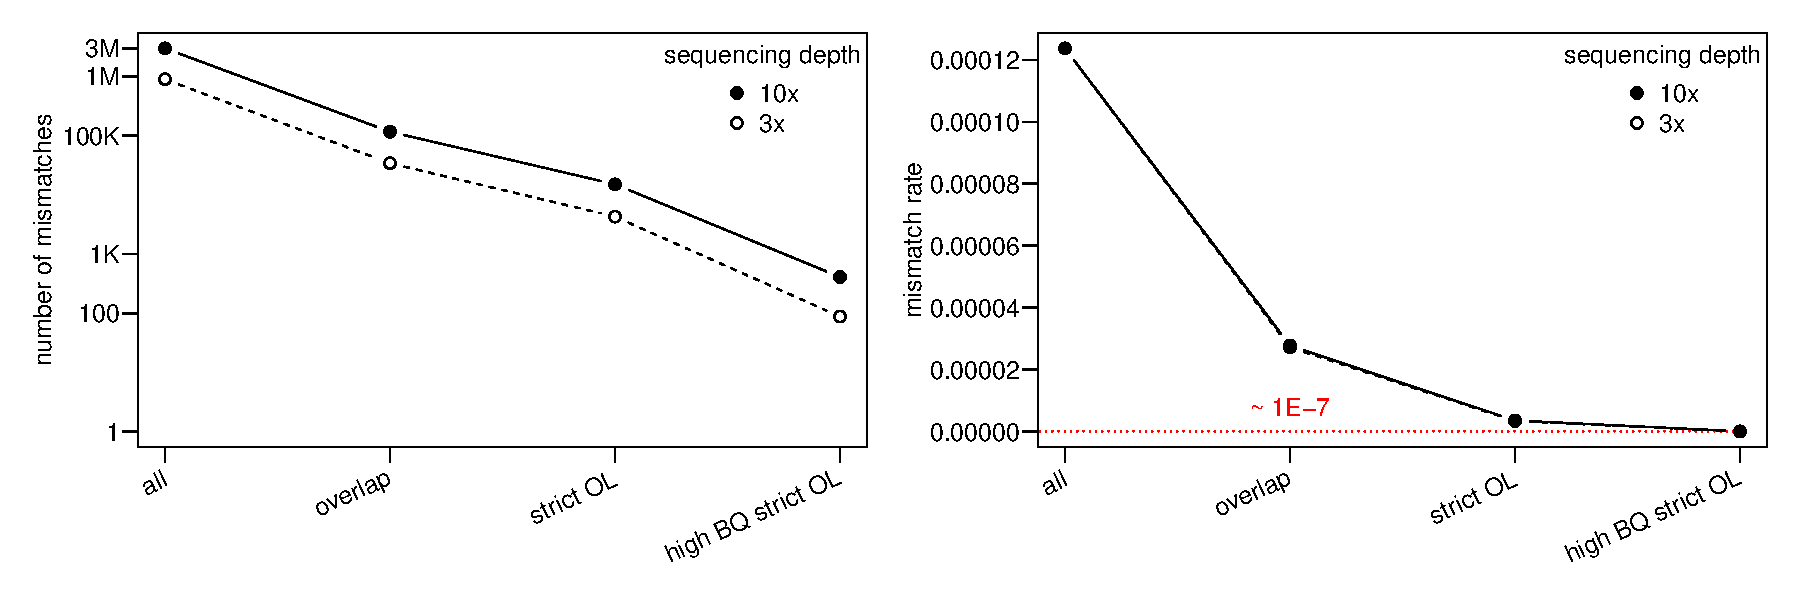
\includegraphics[width=.99\linewidth]{Figures/mismatchrateCleanSequencing.pdf}
\caption[Mismatchrate of different filtering methods]{Mismatchrate of different filtering methods on sequencing data simulated with ART\cite{Huang2011} for both 10x and 3x coverage; Mismatches correspond to simulated sequencing errors; all: no filters, overlap: only use the overlapping parts of paired end reads with consensus building (\protect\autoref{mmf-sec:consensus}), strict OL: overlap but reads \emph{must} agree, high BQ strict OL: strict OL with high BQ in both variants; A) Absolute counts B) counts from A normalised by the number of analysed bases all: all aligned bases, other: number of bases in read overlap}\label{fig:mmf-mismatchrate}
\end{figure}

By only using high base quality mismatches, where both reads agree on the mismatch 99.98\% of all sequencing errors can be eliminated and only 1 in 10M bases will be wrongly counted as a variant (\autoref{fig:mmf-mismatchrate}). This false discovery rate is multiple orders of magnitude lower than before and in a similar range to normal mutationally driven cancers tumour mutational burden \cite{Alexandrov2020,Lawrence2013a}.


\section{Spike-in signature detection}
\label{mmf-sec:simSingnatures}
With the technical error eliminated in simulated data, the question was would our method work in a real world data, however to establish a baseline for detection limit and sensitivity of the method, we decided to first use a hybrid approach, were we spike-in somatic variants into a genuine low coverage WGS sequencing of a healthy control. That reduces the amount of unknown variability from other published datasets.

While it would be possible simulate the variants completely de novo, without any prior knowledge, we know that somatic mutations follow a certain pattern and there a mutational hotspots \cite{Chen2016,Moore2021}, so we decided to instead use the COSMIC database \cite{Tate2018,WSI2021} as the  to select mutations from. This allows us to select mutations, which definitely occurred in a specific cancer subtype, which leads to a simulation which closer resembles real data. The in-depth protocol is shown in \autoref{ch-mmfAppendix:spikein}. The downside of this method is that the spike-in will not predominantly happen on shorter fragments, as it would be the case with ctDNA. 

In the following section I will discuss the results for the simulation of the very prominent SBS7a signature (see \autoref{fig:sig7a})which is predominantly present in Melanoma (see \autoref{mmf-sec:melaSim}) and secondly the much flatter and more uniform SBS3 (see \autoref{A:fig:sig3}), which is a sign of defective homologous recombination in breast cancers (\autoref{mmf-sec:mbcSim})

\subsection{Melanoma - UV exposure}
\label{mmf-sec:melaSim}




\subsection{BRCA1/2 - Defective homologous recombination-based DNA damage repair}
\label{mmf-sec:mbcSim}

\todo[inline]{show data with germline filtering}